By this point in the analysis all the selections have been finalised and discussed.
Furthermore, clear definitions for tag-$B$ mesons that properly kinematically constrain \BtoXsgamma are presented, such that \EB is evaluated accurately.
However, as can be seen \Cref{fig:spectrum_after_optimisation}, even though continuum and $\BB$ backgrounds is suppressed heavily compared to the \EB distributions that was begun with (\Cref{fig:spectrum_after_reco}),
there is still a significantly larger number of background processes than \BtoXsgamma signal events.
Many of these, particularly continuum background, originate from incorrect tag-$B$ mesons (see \Cref{fig:good_tag_definitions}) and can therefore be estimated in data using an \Mbc fitting procedure.
In this section, a thorough overview of the \Mbc fit will be presented which will extract the counts of good-$B$ tags in different \EB intervals.
All shown in this chapter are unbinned extended negative-log likelihood fits, as presented in \Cref{sec:fitting_theory}.


\subsection{Components in the dataset}\label{sec:fitting_components}

There are three types of events in \epem collision dataset following all the selections described so far:
\begin{itemize}
    \item Generic-\BB (including \BtoXsgamma) that are tagged with a good tag-$B$;
    \item Generic-\BB (including \BtoXsgamma) that are tagged with a misreconstructed tag-$B$;
    \item Photons candidates originating in \epem\ra\qqbar.
\end{itemize}
These three components are referred to as `peaking', `combinatorial \BB' and `continuum' throughout this \Cref{sec:fitting_mbc}.
These components, extracted from generic \MC, are visualised in \Cref{fig:tag_component_fits}.

\begin{figure}[htbp!]
    \centering
    \subcaptionbox{\label{fig:good_tags_fit}}{
        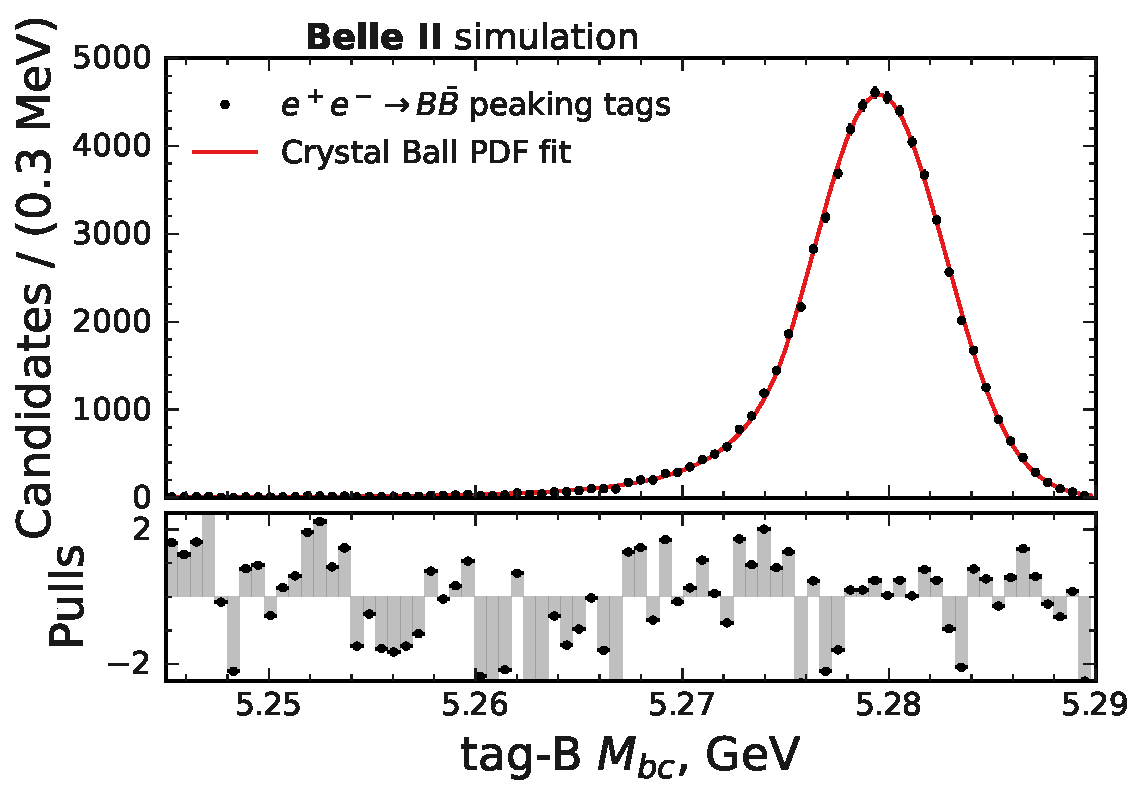
\includegraphics[width=0.3\textwidth]{figures/fitting/mbc_good_tags_fit.pdf}
    }
    \subcaptionbox{\label{fig:combinatorial_tags_fit}}{
        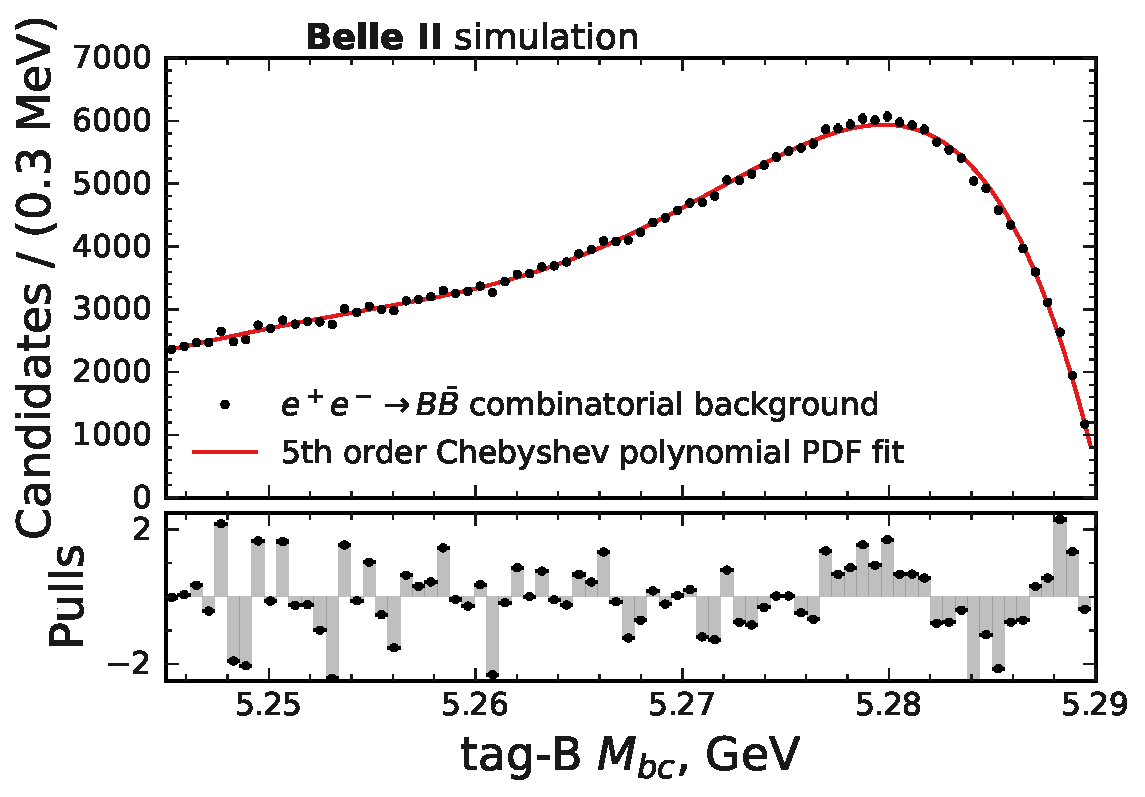
\includegraphics[width=0.3\textwidth]{figures/fitting/mbc_combinatorial_tags_fit.pdf}

    }
    \subcaptionbox{\label{fig:argus_tags_fit}}{
        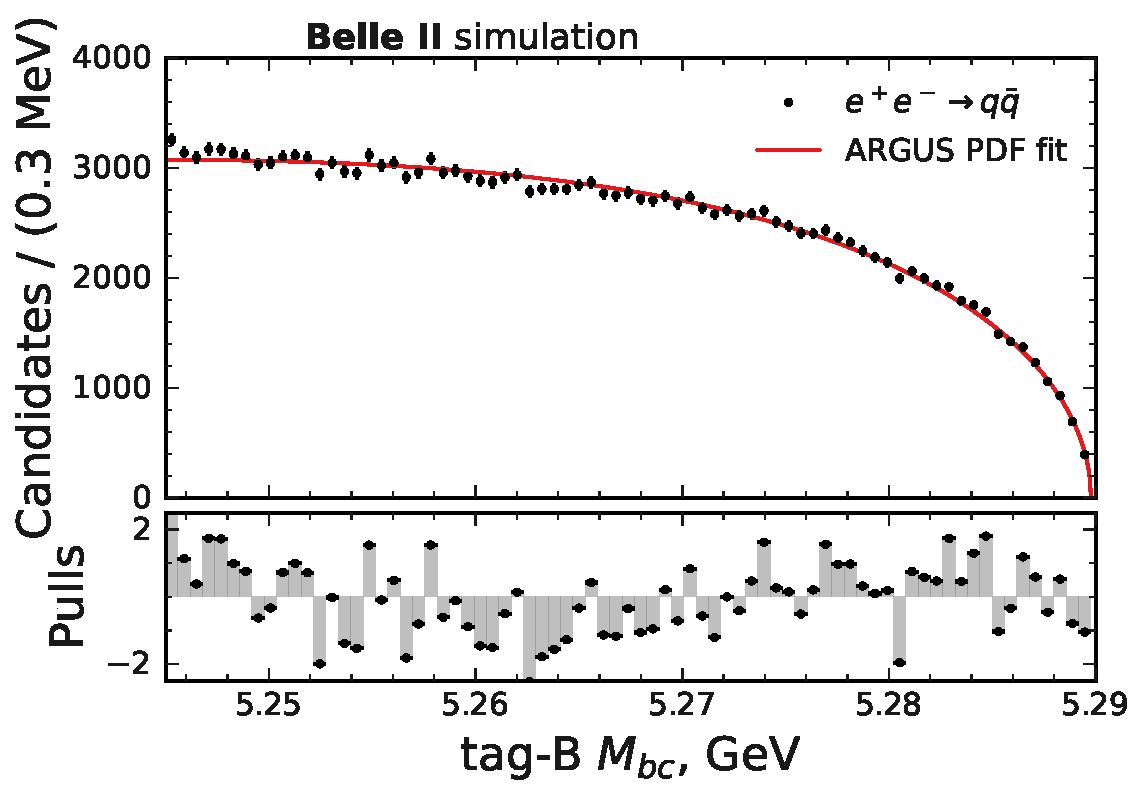
\includegraphics[width=0.3\textwidth]{figures/fitting/mbc_continuum_tags_fit.pdf}
    }
    \caption{\label{fig:tag_component_fits} Separate components that are present in generic \MC after selections that suppress background (\Cref{tab:cutflow}).
    The individual components are defined in \Cref{sec:fitting_components} text.
    Each distribution contains an unbinned illustrative fit to the data points, and the subpanels show the pull (\Cref{eq:pull_distribution}) in each case.
    The fitting function for peaking tag \B mesons (\Cref{fig:good_tags_fit}) is chosen as the Crystal Ball function;
    for combinatorial tag \B mesons (\Cref{fig:combinatorial_tags_fit}) it is chosen as the 5th order Chebyshev;
    for continuum \epem\ra\qqbar events (\Cref{fig:argus_tags_fit}) it is chosen as the ARGUS function.
    }
\end{figure}

The fitting model is prepared to describe the three components and, particularly, to extract the number of tag-$B$ candidates that corresponds to the `peaking' component.
The strategy to describe each component is as follows:
\begin{itemize}
    \item Peaking \Mbc distributions are often fitted using a Crystal Ball function.
    It is defined in \Cref{sec:crystal_Ball}, but can be understood as Gaussia distribution with a polynomial tail.
    \Cref{fig:good_tags_fit} illustrates the suitability to describe the peaking \Mbc distribution.
    \item Continuum \Mbc distributions are conventionally described by the ARGUS function, which is named after the ARGUS collaboration and designed specifically for this purpose;
    This function, utilised to describe \epem\ra\qqbar simulated backgrounds in this analysis is seen in \Cref{fig:argus_tags_fit}.
    \item The particular shape of the combinatorial \BB background is generally dependant on the signal mode and do not have a conventional method of description.
    In this analysis, the usage of \FEI and the fact that background events are conservatively suppressed to avoid signal-side biases leads to an wide but slightly peaking shape.
    Several options were assessed in this ana;lysis, but it was found that it is suitably described by a Chebyshev polynomial, which can be adapted to a necessary functional shape.
    This is illustrated in \Cref{fig:combinatorial_tags_fit}, where a 5th order polynomial describes the combinatorial \BB background distribution.
\end{itemize}
In \Cref{fig:tag_component_fits} the subpanels shown the pull distribution, which is defined as:
\begin{equation}\label{eq:pull_distribution}
    \mathrm{pull}(x) = \frac{x-\mu}{\sigma}. 
\end{equation}
Throughout this thesis it is used to evaluate the quality of the fit, as repeated measurements of a random variable $x$ should fluctuate around a mean value $\mu$ with a possonian width $\sigma$.
Therefore any dependancies or strucutes observed in the pull distribution would be indicators of poor fit quality. 

\subsection{Photon energy intervals for the fit}\label{sec:binning}

It is clear from \Cref{fig:spectrum_after_optimisation} that signal-to-background ratio changes across all \EB range.
In fact, even continuum-to-\BB event fractions are not constant.
This is a result of the fact that photons related to \epem\ra\qqbar backgrounds are more likely to extend to high-\EB values, because they do not originate from a \B meson which is always produced with $\sqrt{s}/2$ at Belle II.
The goal of the fit, as discussed in the introduction of this Section, is to remove combinatorial \BB and continuum events from further analysis.
While an overall \Mbc fit could be performed, such an approach necessarily loses event-level information, such as the energy of each individual photon, and only provides the event-counts in the fitted \EB region.
Furthermore, the fact that the background composition is expected to vary with \EB, such an overall-fit may generally be suboptimal.

Instead, in this analysis the photon spectrum is divided into multiple \EB intervals, and the \Mbc distributions belonging to each interval are fitted using the functions described in \Cref{sec:fitting_components}.
This approach will then reduce the existing dataset to multiple \EB intervals with known good tag-\B counts, completely removing continuum and combinatorial \BB events from the dataset.
Such an approach means that the final photon-energy spectrum will be provided in the binning used for fitting.
It is therefore important to optimise the chosen intervals for the fit with respect to expected \BtoXsgamma in each interval, despite the fact that the primary goal of the fit is not signal extraction.
For the rest of the thesis, \EB intervals will be referred to as \EB bins.

Three scenarios are tested for $\EB\in(1.4,2.8)~\gev$: 50~\mev, 100~\mev and 200~\mev wide bins.
The test is performed by evaluating the statistical significance, with a definition equivalent to \Cref{eq:soversqrtsplusb}, on a dataset scaled to 200~\invfb.
In this case, the background is considered what is anticipated after the \Mbc fit: only correctly-tagged \BB events (no combinatorial or continuum background).
The result of the study of statistical significance for the hybrid signal model (\Cref{sec:signal_model}) is shown in \Cref{fig:binning_significance}.

\begin{figure}[htbp!]
    \centering
    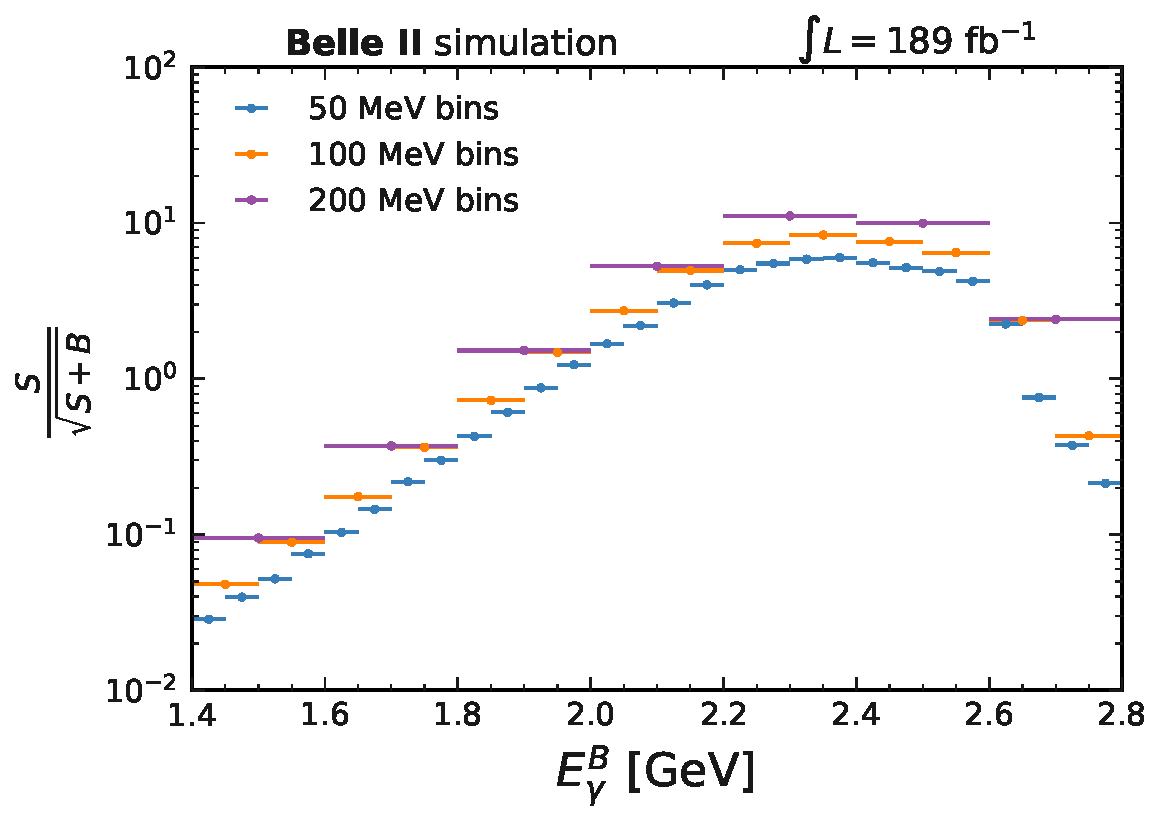
\includegraphics[width=0.5\textwidth]{figures/fitting/binning_significance.pdf}
    \caption{\label{fig:binning_significance}The results of statistical significance, based on \Cref{eq:soversqrtsplusb}.
    Here the $S$ is takes as number of \BtoXsgamma events after fitting and $B$ is taken as non-\BtoXsgamma events expected after fitting in each \EB interval.
    Three scenarios are tested: 50~\mev, 100~\mev and 200~\mev wide bins.
    The final binning chosen is a hybrid scenario described in \Cref{sec:binning} text.
    The hybrid model described in \Cref{sec:signal_model} is used for this study.
    }    
\end{figure}

In general, the highest statistical significance is observed with the widest bins, but this method, by definition, contains the least amount of information about the spectrum.
Irrespective of the bin-width,  $\EB\in(1.4,1.8)$ and $\EB>2.6$ show a statistical significance lower than unity, therefore the selected binning should attempt to maximise it.
In the case of $\EB\in(1.8,2.0)$ bin, it is observed that a similar statistical significance can be achieved a with $\EB\in(1.9,2.0)$ bin.
This motivates to extend it, such that an \EB threshold of 1.8~\gev could be achieved, as opposed to the 1.9~\gev threshold in Ref.\cite{BaBar:2007yhb}.
Later studies performed in \Cref{sec:resolution_studies} showed that the resolution of \EB is expected to be roughly $30-40~\mev$.
The coarse intervals of \EB compared to the resolution may lead to complications in the unfolding procedure.
As the simpler bin-by-bin unfolding is employed in this analysis, the 50~\mev bins were not considered.

These considerations led to choosing the following eleven \EB bins for the analysis:
\begin{itemize}
    \item Three 200~\mev bins for $\EB\in(1.4,2.0)$;
    \item Seven 100~\mev bins for $\EB\in(2.0,2.7)$;
    \item A single, inclusive overflow bin $\EB>2.7$.
\end{itemize}
This choice provides a compromise between statistical significance, \EB spectrum resolution and complications in unfolding.
The expected continuum, combinatorial, correctly-tagged non-\BtoXsgamma $BB$ and correctly-tagged \BtoXsgamma event count expectations for the chosen binning are provided in \Cref{tab:expected_events}.
Note that the table entry containing combinatorial tag-\B backgrounds, may include events where \BtoXsgamma events are present.
However, it is  necessarily rejected as background in the \Mbc fits in \Cref{sec:fitting_mbc}.
On the other hand peaking-\BB background, which is not rejected by the \Mbc fit and will be treated in \Cref{sec:background_subtraction}, is separated from \BtoXsgamma.
The table also highlights the importance of a correct binning, as it is obvious that several bins are able to achieve a comparable statistical significance to the one that could be achieved if just a single bin was used.

\begin{table}[htbp!]
    \caption{\label{tab:expected_events}Expected number of events as a fraction of the dataset after selections in \Cref{tab:cutflow}, for the binning chosen in \Cref{sec:binning}.
    The table also shows corresponding statistical significance for a 189~\invfb sized dataset.
    }
    \resizebox{1\textwidth}{!}{
\begin{tabular}{|l|lllll|}
\hline
\EB bins [\gev] & Continuum frac. & Combinatorial \BB (incl. \BtoXsgamma) & Peaking \BB frac (excl. \BtoXsgamma) & Peaking \BtoXsgamma & $\frac{S}{\sqrt{S+B}}$ at 189~\invfb \\
\hline
$1.4-1.6$ &    0.22 &       0.20 &   0.047 &  0.00010 & 0.1 \\
$1.6-1.8$ &    0.14 &      0.094 &   0.028 &  0.00031 & 0.38 \\
$1.8-2.0$ &    0.088 &      0.046 &   0.016 &   0.00097 &  1.56 \\
$2.0-2.1$ &   0.028 &      0.013 &  0.0048 &   0.0010 &    2.80 \\
$2.1-2.2$ &    0.020 &     0.0079 &  0.0026 &   0.0016 &  5.05 \\
$2.2-2.3$ &   0.013 &     0.0048 &   0.00093 &   0.0019 &  7.5 \\
$2.3-2.4$ &  0.0075 &     0.0033 &  0.00031 &    0.0019 &   8.4 \\
$2.4-2.5$ &  0.0042 &     0.0019 &  0.00024 &   0.0015 &   7.6 \\
$2.5-2.6$ &  0.0019 &    0.00062 &  0.00013 &    0.0011 &  6.5 \\
$2.6-2.7$ & 0.00059 &    0.000098 & 0.000016 &  0.00014 &  2.38 \\
$2.7-5.0$ & 0.00021 &     0.000011 &   $<0.000001$ &  0.000005 & 0.46 \\
\hline
All        &    0.52 &       0.37 &    0.10 &    0.011     &   6.61 \\
\hline
\end{tabular}
}
\end{table}

Because of the low expected statistical significance, the $\EB\in(1.4,1.8)$ and $\EB>2.7~\gev$ are chosen as validation regions.
They will later be referred to as \textit{sidebands}.
Consequentially, the signal region of the study is defined as $\EB\in(1.8,2.7)$.

\subsection{\texorpdfstring{\Mbc}{Mbc} fit model building}\label{sec:fitting_setup}

The functions introduced in \Cref{sec:appendix_fitting_functions} are now considered in terms of the defined binning in \Cref{sec:binning}.
Using them a \Mbc parameter estimation (fit) model for the total dataset build.
However, the implementation of an $N$-th order Chebyshev polynomial, a Crystal Ball function and an ARGUS function for every \EB bin is unreasonable:
this would result in $N+6$ model parameters and 3 normalisation parameters for each bin.
Therefore, first, a fit model version, where some of the parameters can be pre-determined or shared amongst the bins is prepared.
This is discussed in \Cref{sec:crystal_ball_prefit,sec:chebyshev_prefit,sec:argus_prefit}.
The key idea is that all the functions are fitted once, separately, on the subsets of the simulated data that they aim to describe.
This is done in order to estimate the starting parameters that will be used on the fit of the total (combined) dataset.
Then, certain fitting parameters are grouped together, such that a simultaneous determination with some parameters shared across multiple bins is prepared.

The key points of the aforementioned subsections and the final fitting model for the analysis is summarised in \Cref{tab:fitting_init_params}.
This fitting model will then be applied on the total dataset in \Cref{sec:mbc_fit_full_mc} in order to estimate the main parameter of interest: normalisations of the Crystal Ball in every \EB bin (i.e. number of good tags in each \EB bin.)
The primary \Mbc fits determining the parameters from \Cref{tab:fitting_init_params} on correspondign datasets are given in \Cref{sec:appendix_primary_fits}. 

\begin{table}[htbp!]
    \centering
    \caption{\label{tab:fitting_init_params} The summary of the fitting model used in this analysis for the \Mbc fit.
    The paramaters are initialised at the values that are listed, corresponding to the ones determined in the primary fitting steps, explained in \Cref{sec:crystal_ball_prefit,sec:chebyshev_prefit,sec:argus_prefit}.
    The values that are bolded in the table are not estimated from the final \Mbc fit, but are kept at their initialised values.
    On the other hand, all non-bolded values are estimated from the final fitter.
    The uncertainties are those estimated using the \texttt{HESSE} method.
    }
\resizebox{1\textwidth}{!}{
    {\def\arraystretch{1.5}\tabcolsep=5pt
        \begin{tabular}{|c|c|c|c|c|c|c|c|c|c|c|c|}

            \multicolumn{12}{c}{Fitting model} \\
            \hline
            \multirow{2}{*}{\EB bin} & \multicolumn{4}{|c|}{Crystal Ball} & \multicolumn{5}{c|}{Chebyshev}    & \multicolumn{2}{c|}{Argus} \\
            \cline{2-12}
                                    & $\mu$ & $\sigma$ & $\alpha$ & $n$    & $k_1$ & $k_2$ & $k_3$ & $k_4$ & $k_5$ & $c$ & $m_0$                 \\
            \hline
            1.4 -- 1.6               & \multirow{11}{*}{$5.27946\pm0.00002$} & \multirow{11}{*}{$0.00302\pm0.00002$} & \multirow{11}{*}{$1.573\pm0.035$} & \multirow{11}{*}{$3.568\pm0.22$} & $-0.0751\pm0.0071$ & $-0.3125\pm0.0073$ & $-0.2516\pm0.0064$ & $-0.1381\pm0.0064$  & $-0.0296\pm0.0062$  &  $-33.11 \pm    0.79$ & \multirow{11}{*}{$5.2897719 \pm 0.0000006$} \\
            \cline{1-1}\cline{6-11}
            1.6 -- 1.8               &                                      &                                        &                                   &                                  & $-0.01 \pm 0.01$ & $-0.33\pm0.01$ & $-0.283 \pm  0.009$ & $-0.143\pm0.009$ & $-0.033\pm0.009$ & $-28.03 \pm 1.00$ & \\               
            \cline{1-1}\cline{6-11}
            1.8 -- 2.0               &                                      &                                        &                                   &                                  & \multirow{9}{*}{$0.119\pm0.011$} & \multirow{9}{*}{$-0.362\pm0.012$} & \multirow{9}{*}{$-0.348\pm 0.010$} & \multirow{9}{*}{$-0.193\pm0.010$} & \multirow{9}{*}{$-0.029 \pm 0.010$} & \multirow{9}{*}{$-25.07 \pm 0.92$} & \\                         
            \cline{1-1}
            2.0 -- 2.1               &                                      &                                        &                                   &                                  &                 &                  &                   &                  &                    &                   & \\                                                                  
            \cline{1-1}
            2.1 -- 2.2               &                                      &                                        &                                   &                                  &                 &                  &                   &                  &                    &                   & \\   
            \cline{1-1}
            2.2 -- 2.3               &                                      &                                        &                                   &                                  &                 &                  &                   &                  &                    &                   & \\   
            \cline{1-1}
            2.3 -- 2.4               &                                      &                                        &                                   &                                  &                 &                  &                   &                  &                    &                   & \\   
            \cline{1-1}
            2.4 -- 2.5               &                                      &                                        &                                   &                                  &                 &                  &                   &                  &                    &                   & \\   
            \cline{1-1}
            2.5 -- 2.6               &                                      &                                        &                                   &                                  &                 &                  &                   &                  &                    &                   & \\   
            \cline{1-1}
            2.6 -- 2.7               &                                      &                                        &                                   &                                  &                 &                  &                   &                  &                    &                   & \\   
            \cline{1-1}
            2.7 -- 5.0               &                                      &                                        &                                   &                                  &                 &                  &                   &                  &                    &                   & \\   
            \hline
        \end{tabular}
    }
}

\end{table}

\subsubsection{Crystal Ball function}\label{sec:crystal_ball_prefit}

The Crystal Ball function, describes the distribution of `good' tag-\B mesons in \Mbc in terms of parameters $\mu$, $\sigma$, $\alpha$ and $n$ and the normalisation of the \PDF $\mathcal{N}$ (see \Cref{eq:crystal_ball}).
In principle, the tag-\B meson is an independent object from the signal-\B meson decays -- which means that no strong \EB correlation is expected.
This hypothesis is tested in \Cref{fig:crystal_ball_par_test}.
It can be seen that strong correlations between \EB and parameters $\mu$ and $\sigma$ are absent.
This test is not performed on parameters $\alpha$ and $n$, as they tend to be less-stable than $\mu$ and $sigma$ and depend more on fluctuations of the dataset.
It is therefore concluded, that a single \Mbc shape for \EB bins will be used, with the parameters pre-determined in a total fit (\Cref{fig:good_tags_fit}).
The normalisations, on the other hand, will be determined for each \EB interval during the total fit.
The values and uncertainties from the fitter, are shown in \Cref{tab:fitting_init_params}.

\begin{figure}[htbp!]
    \subcaptionbox{\label{fig:crystal_ball_mus}}{
        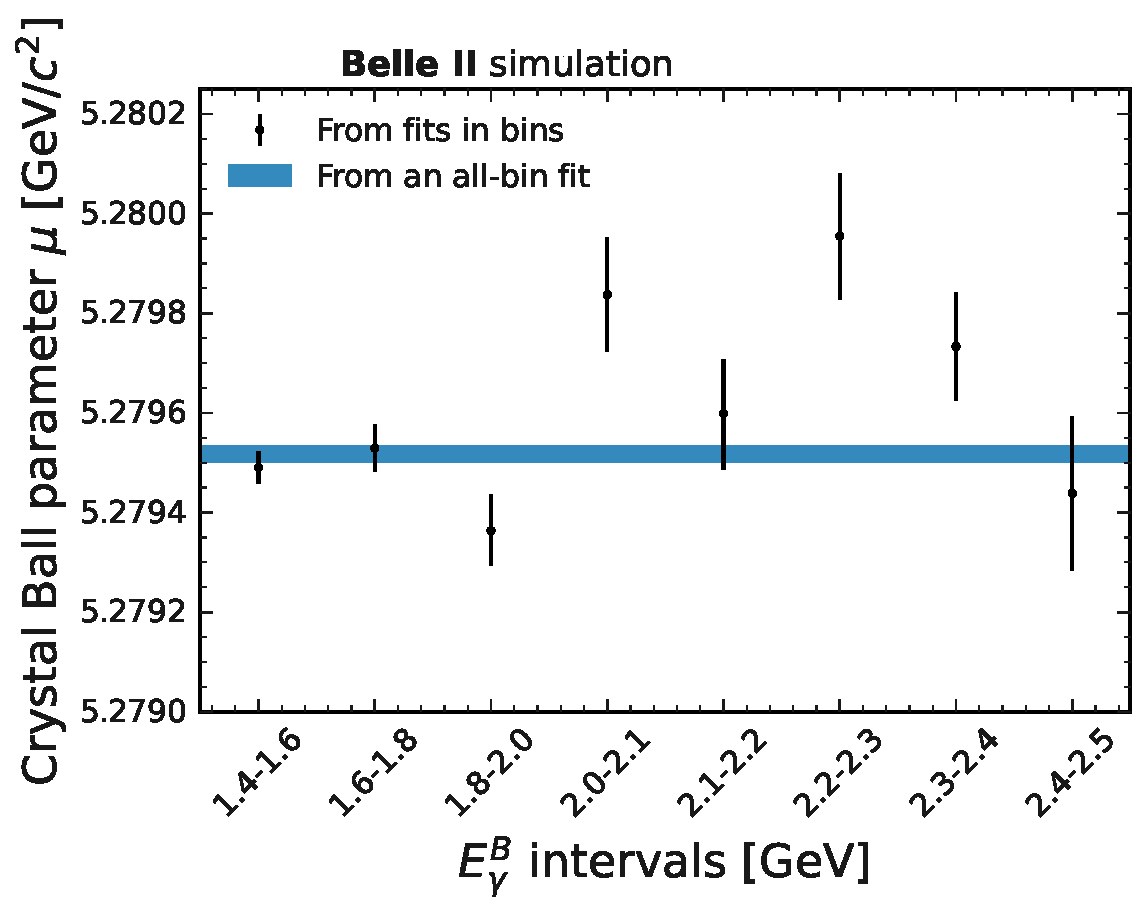
\includegraphics[width=0.4\textwidth]{figures/fitting/Crystal_Ball_PDF_test_mu.pdf}
    }
    \subcaptionbox{\label{fig:crystal_ball_sigmas}}{
        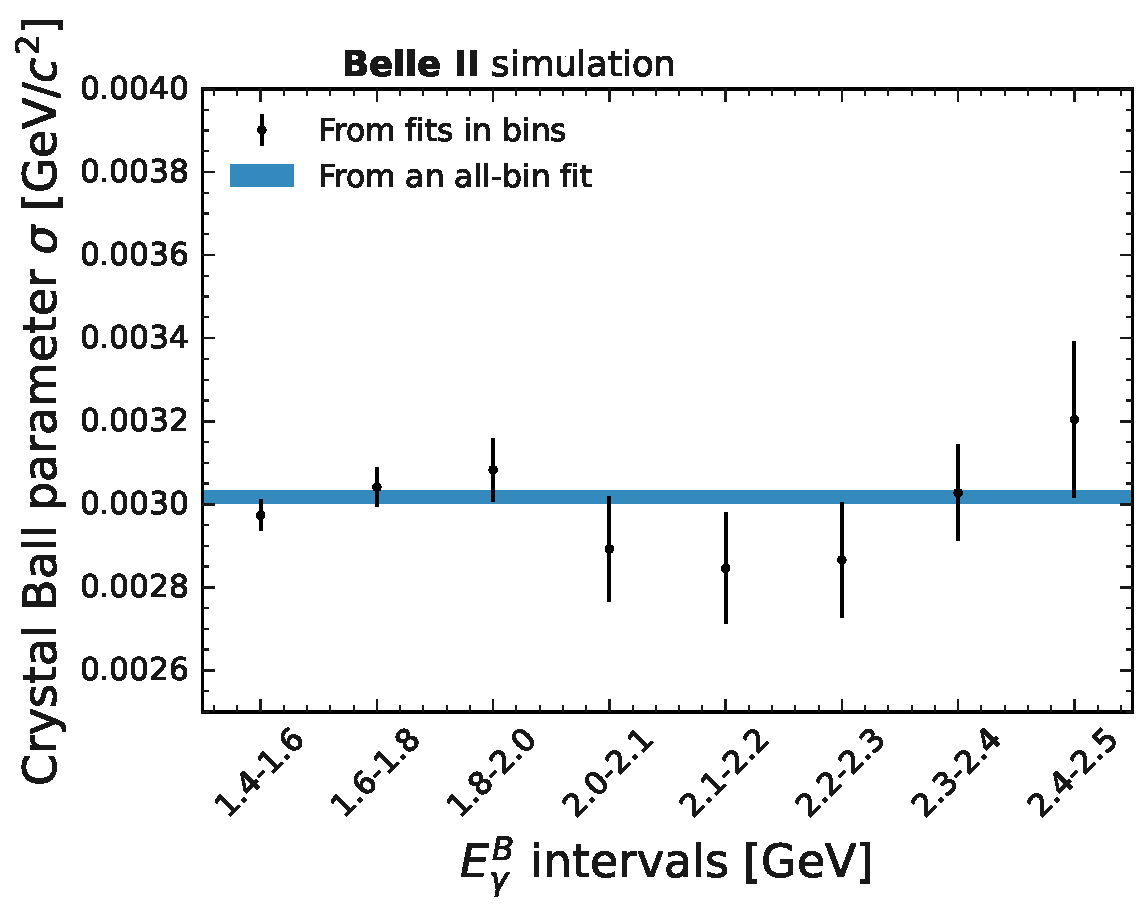
\includegraphics[width=0.4\textwidth]{figures/fitting/Crystal_Ball_PDF_test_sigma.pdf}
    }
    \caption{\label{fig:crystal_ball_par_test}The parameters from \Mbc fits of `good' tag-\B mesons in generic-\BB simulation, using a Crystal Ball function.
    The datapoints showcase the estimated parameters $\mu$ (\Cref{fig:crystal_ball_mus}) and $\sigma$ (\Cref{fig:crystal_ball_sigmas}) for different
    \EB intervals.
    This can be compared with the overall shape (blue band), that is determined if the entire $\EB\in(1.4,2.8)$ region is fitted.
    The parameters of the blue band correspond to the fit in \Cref{fig:good_tags_fit}.
    No strong dependance on \EB is observed.
    }
\end{figure}

\subsubsection{Chebyshev polynomial function}\label{sec:chebyshev_prefit}

The Chebyshev \PDF takes $N$ parameters as coefficients scaling each order of the polynomial that goes into the fitting function, and a normalisation $\mathcal{N}$ (\Cref{eq:chebyshev_pdf}).
The $N$ is therefore referred to as the \textit{order} of the Chebyshev \PDF.
3-rd, 4-th and 5-th order Chebyshev polynomials are tested for suitability to describe the combinatorial \BB background distribution.
The 5-th order result is already introduced in \Cref{fig:combinatorial_tags_fit}.
The results of the best fit for lower-order polynomials is presented in \Cref{fig:lower_order_chebyshev}.
From the pull distributions in the subpanels and the general inspection of the fit, it is clear that using a polynomial of order lower than 5 is insufficient for an adequate description of combinatorial \BB events.

\begin{figure}[htbp!]
    \centering
    \subcaptionbox{\label{fig:3rd_order_chebyshev}}{
        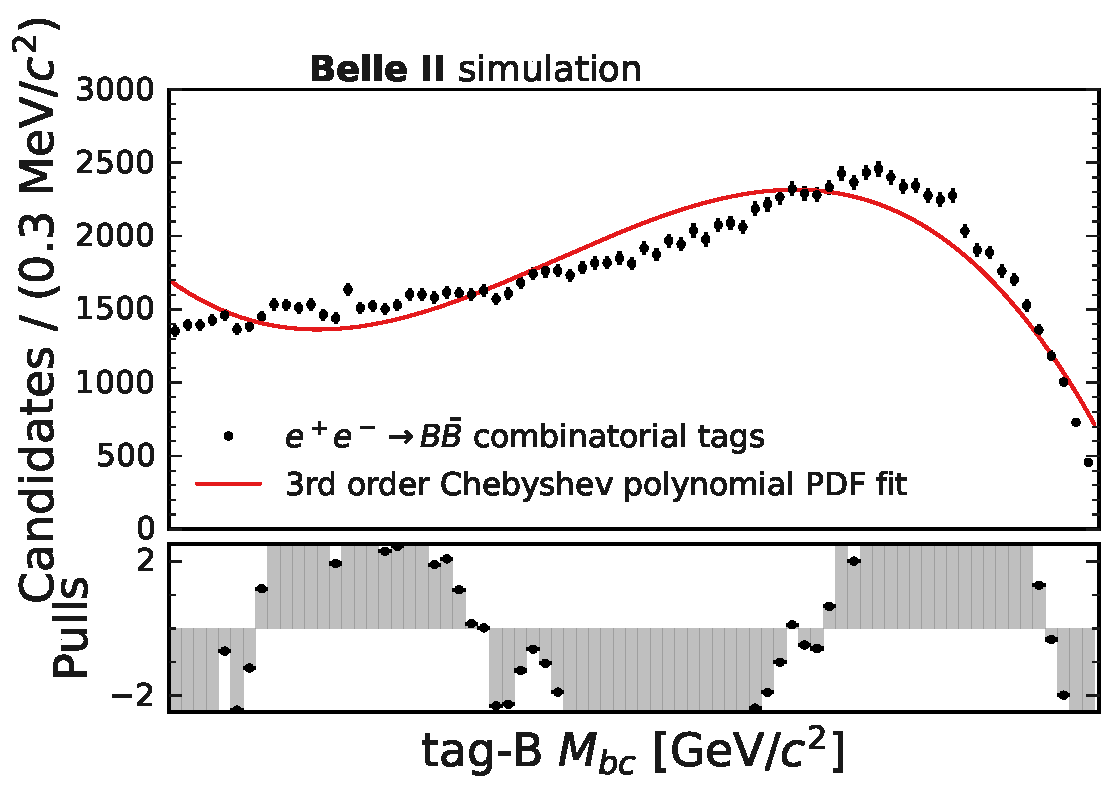
\includegraphics[width=0.4\textwidth]{figures/fitting/3rd_order_chebyshev_polynomial.pdf}
    }
    \subcaptionbox{\label{fig:4th_order_chebyshev}}{
        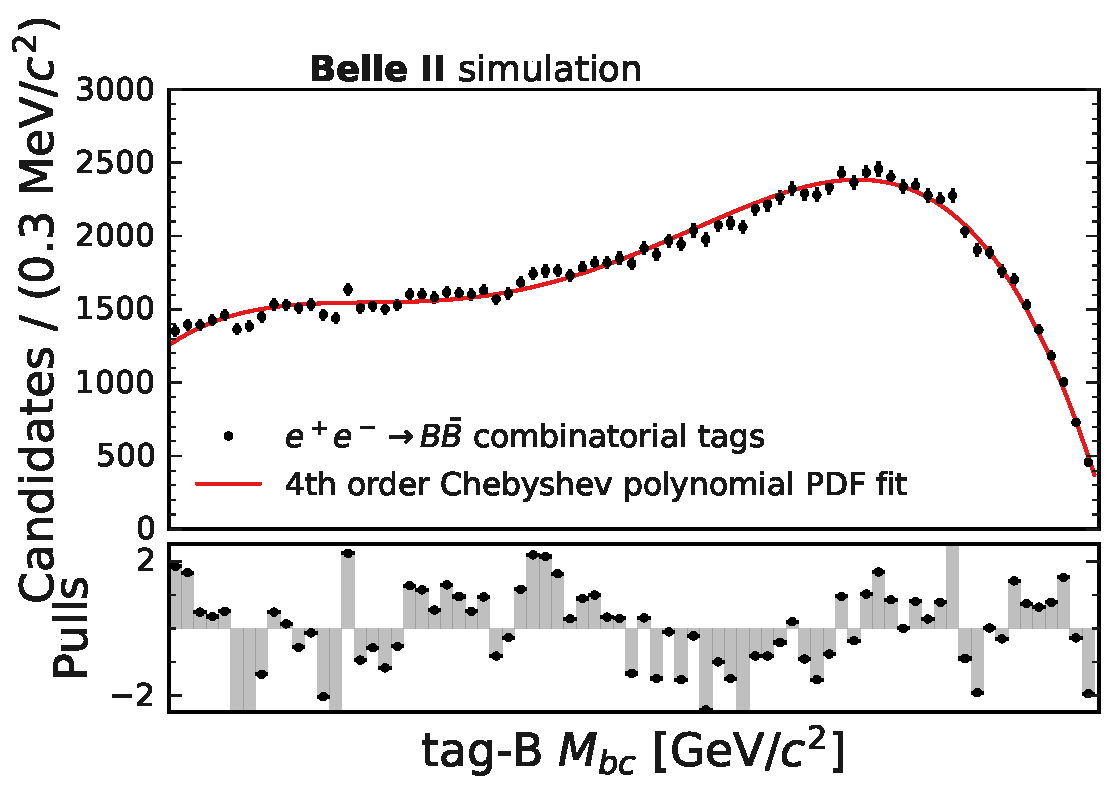
\includegraphics[width=0.4\textwidth]{figures/fitting/4th_order_chebyshev_polynomial.pdf}
    }
    \caption{\label{fig:lower_order_chebyshev}The \Mbc fits of combinatorial \BB events when a Chebyshev \PDF of order 3 (\Cref{fig:3rd_order_chebyshev}) or 4 (\Cref{fig:4th_order_chebyshev}) is used.
    These figures can be compared to \Cref{fig:combinatorial_tags_fit}.
    It is clear that lower order Chebyshev polynomials are unable to accurately describe the combinatorial-\BB data.
    }
\end{figure}


The coefficients $k_{1-5}$ of the Chebyshev polynomial cannot be easily connected to physics observables,
and therefore it is hard to evaluate their dependance on \EB.
As such, 3 different Chebyshev PDFs are evaluated for the following intervals: $\EB\in(1.4,1.6)$, $\EB\in(1.6,1.8)$, $\EB>1.8$ \gev.
The reason why the last interval is not subdivided further is because of the dataset size (see \Cref{tab:expected_events}) -- each interval was optimised to have a roughly equal number of events, to minimize statistical fluctuations related to the shape determination.
The Chebyshev \PDF parameters for each interval are determined in an \Mbc fit on the appropriate region and fixed for the fit of the total dataset later.
The normalisations will be determined for each \EB interval during the total fit.
The initial values for the total fitter, determined in an \Mbc fit on combinatorial \BB events in generic \MC, on the defined \EB binning and fitting intervals, is presented in \Cref{tab:fitting_init_params}.

\subsubsection{ARGUS function}\label{sec:argus_prefit}

Similarly to the previous cases, the ARGUS function has 2 parameters, $c$ and $m_0$, and a normalisation $\mathcal{N}$ (\Cref{eq:argus_function}).
Unlike the coefficients of the Chebyshev, the $c$ and $m_0$ are easier to understand intuitively: with $m_0$ corresponding to max \Mbc values in the distribution and $c$ to the shape of continuum background.
More generally, the variation of $c$ and $m_0$ can allow to account for possible background-shape differences between the simulation and data.
It offers an additional layer of flexibility, through a variation of relative ARGUS and Chebyshev normalisation values.
This means, that allowing a degree of variation in the ARGUS functions is beneficial to account for possible background shape differences.

Following these considerations, a similar setup is adopted, with independent shapes for  $\EB\in(1.4,1.6)$, $\EB\in(1.6,1.8)$, $\EB>1.8$ \gev.
Unlike for the previous two components, in each respective range one single shape parameter $c^{(1.4-1.6)}$, $c^{(1.6-1.8)}$, $c^{(>1.8)}$ is determined from the total fit.
To account for possible endpoint differences (differences between simulated and data $\sqrt{s}$), the $m_0$ parameter is shared accross all bins and is also determined from the fit of the combined dataset.
The discussed fits are performed simultaneously on continuum \Mbc distributions in all \EB bins.
The initial values for the total fitter, determined in an \Mbc fit on continuum events in generic \MC, on the defined \EB binning and fitting intervals, is presented in \Cref{tab:fitting_init_params}.


\subsection{\texorpdfstring{\Mbc}{Mbc} fit on the total simulated dataset}\label{sec:mbc_fit_full_mc}

The prepared fitter, discussed in \Cref{sec:fitting_setup}, is applied on the total generic \MC dataset.
The initial values of the fit are given in \Cref{tab:fitting_init_params} and all bins are fitted simultaneously.
The fit results are shown in \Cref{fig:primary_full_fits}.
The overall \Mbc distributions are accurately described accross all \EB bins, irrespective of the overall number of data points that are being fitted.
This is already an important achievement -- as a single fitting setup is adaptive enough to cover different signal-to-background ratios, statistical sample size, and overall shape of the distributions.

\begin{figure}[htbp!]
    \centering
    \subcaptionbox{\label{fig:mbc_full_1p4}}{
        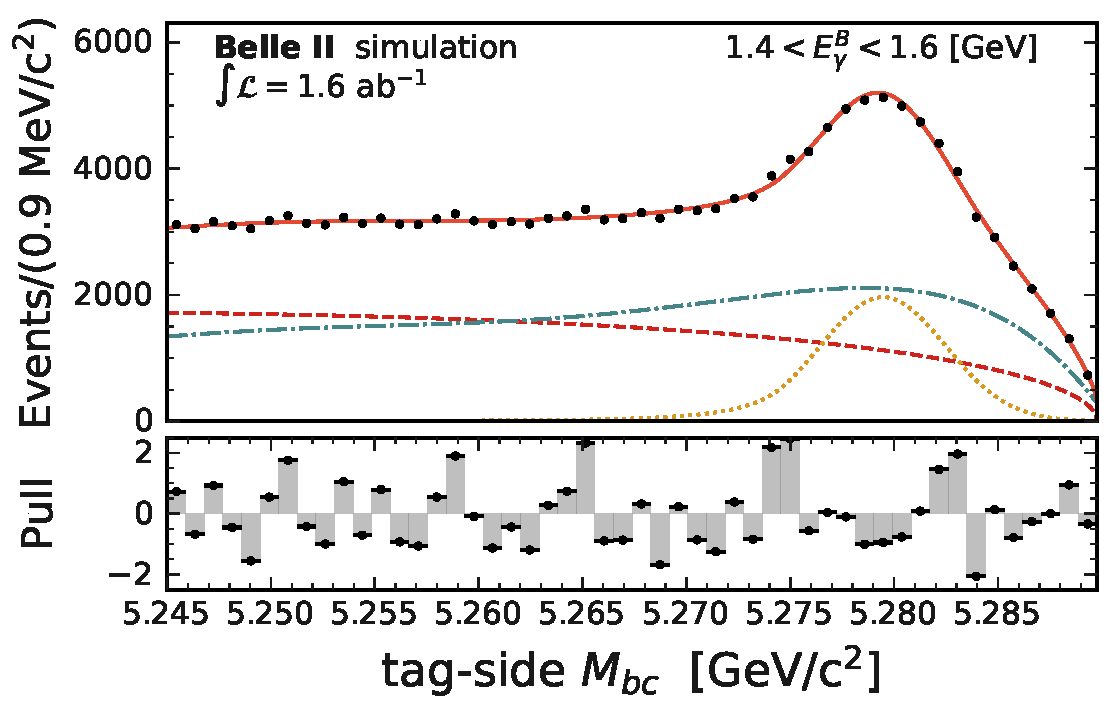
\includegraphics[width=0.3\textwidth]{figures/fitting/fits/full_MbcFit_1p4to1p6ppdf.pdf}
    }
    \subcaptionbox{\label{fig:mbc_full_1p6}}{
        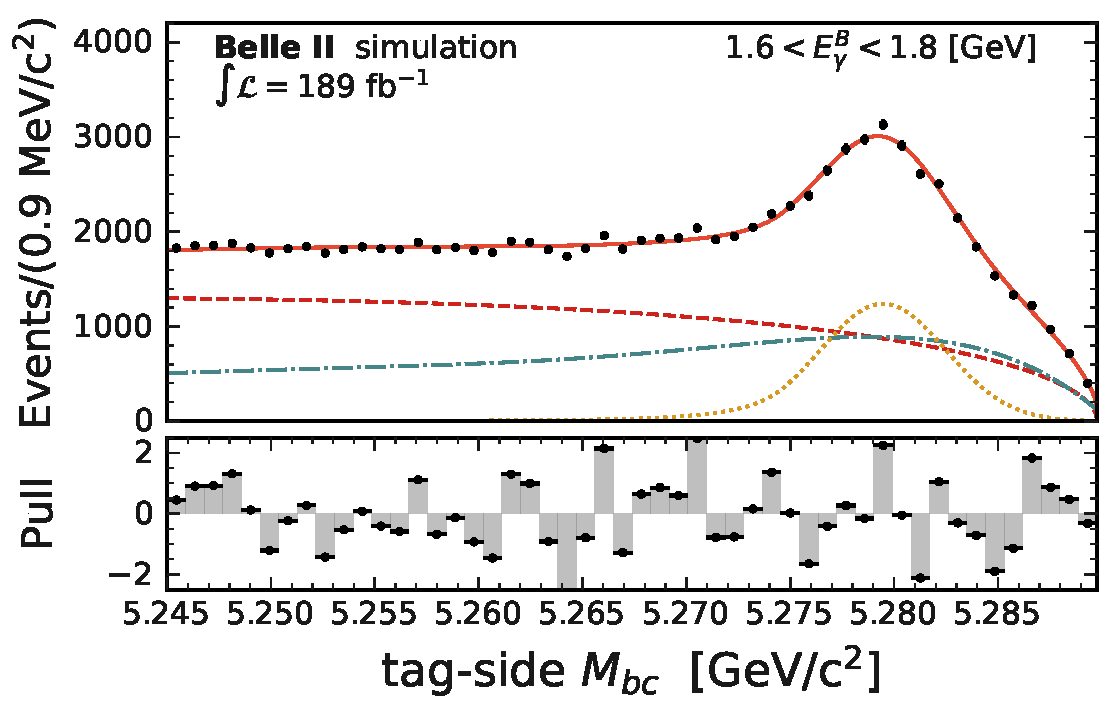
\includegraphics[width=0.3\textwidth]{figures/fitting/fits/full_MbcFit_1p6to1p8ppdf.pdf}
    }
    \subcaptionbox{\label{fig:mbc_full_1p8}}{
        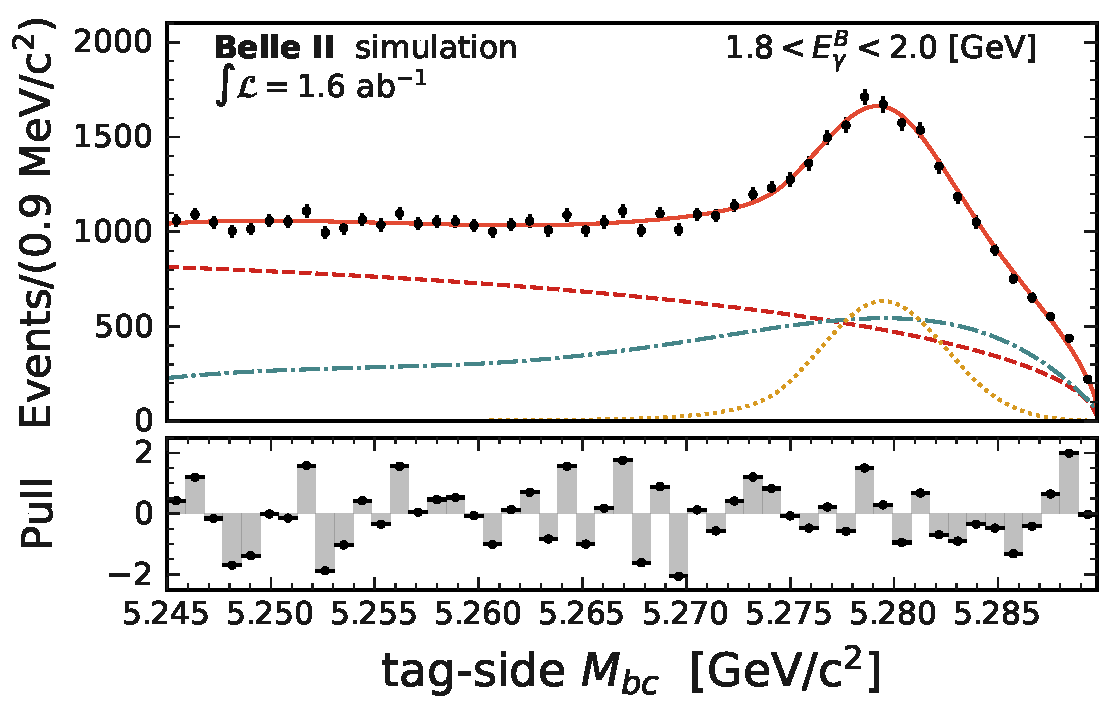
\includegraphics[width=0.3\textwidth]{figures/fitting/fits/full_MbcFit_1p8to2p0ppdf.pdf}
    }
    \subcaptionbox{\label{fig:mbc_full_2p0}}{
        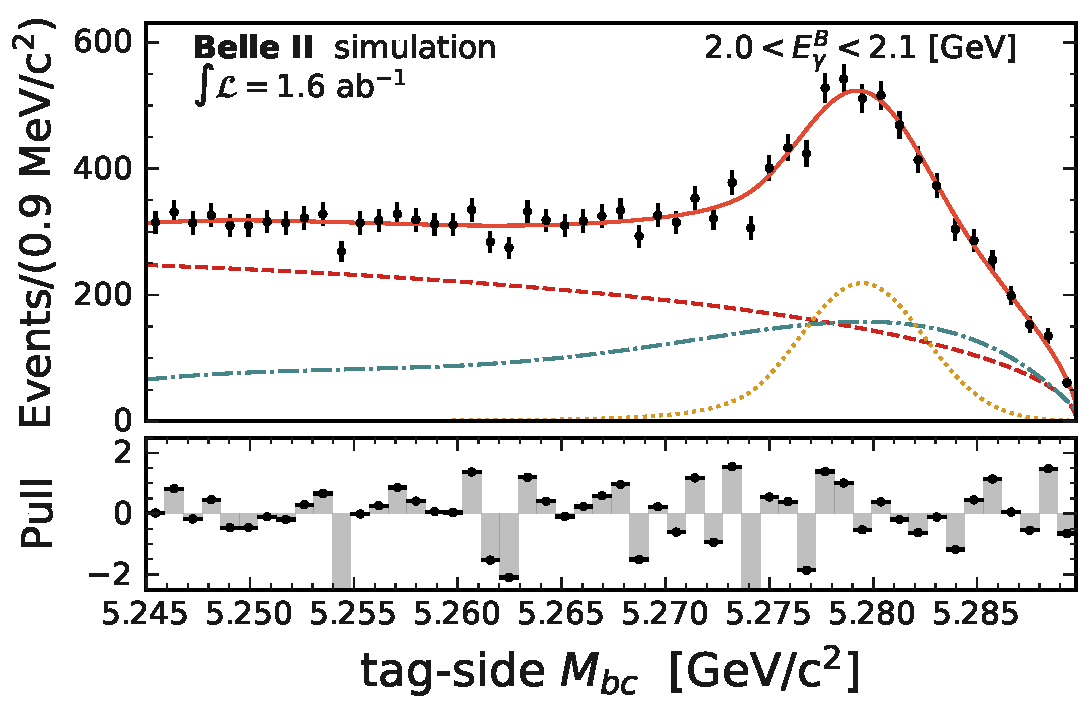
\includegraphics[width=0.3\textwidth]{figures/fitting/fits/full_MbcFit_2p0to2p1ppdf.pdf}
    }
    \subcaptionbox{\label{fig:mbc_full_2p1}}{
        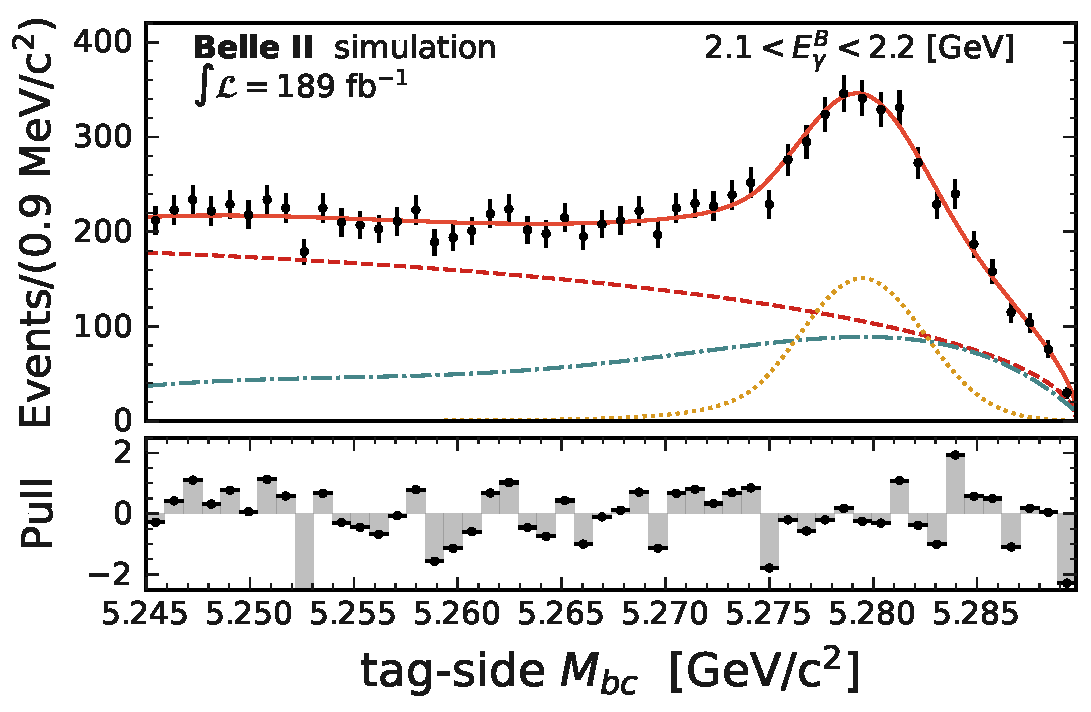
\includegraphics[width=0.3\textwidth]{figures/fitting/fits/full_MbcFit_2p1to2p2ppdf.pdf}
    }
    \subcaptionbox{\label{fig:mbc_full_2p2}}{
        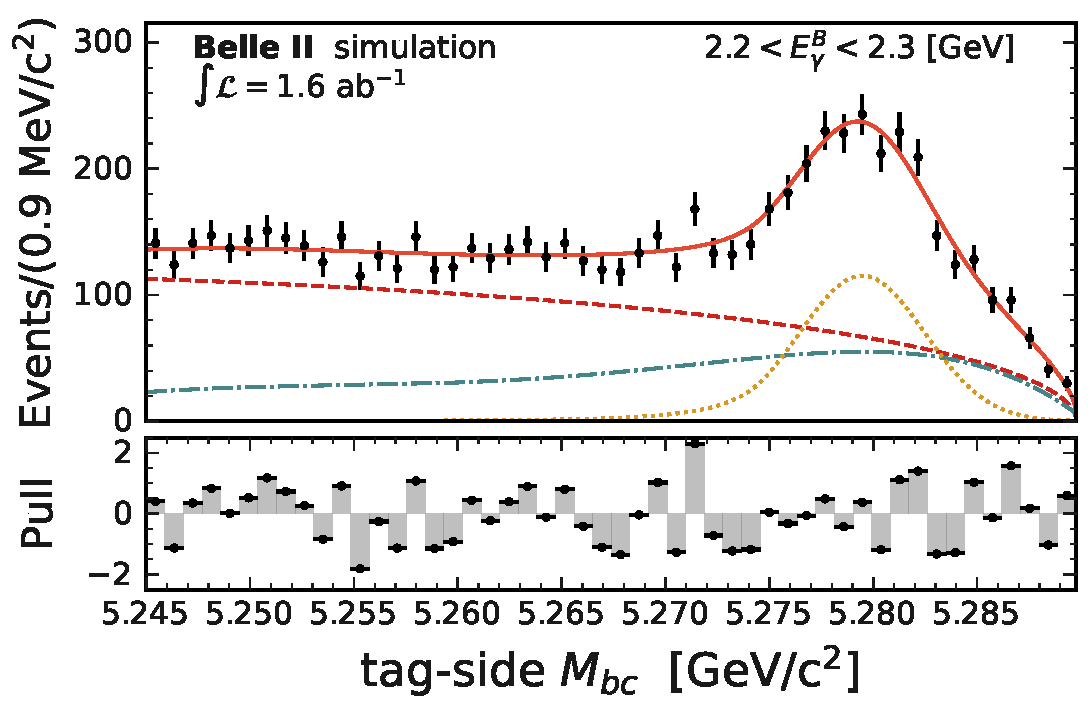
\includegraphics[width=0.3\textwidth]{figures/fitting/fits/full_MbcFit_2p2to2p3ppdf.pdf}
    }
    \subcaptionbox{\label{fig:mbc_full_2p3}}{
        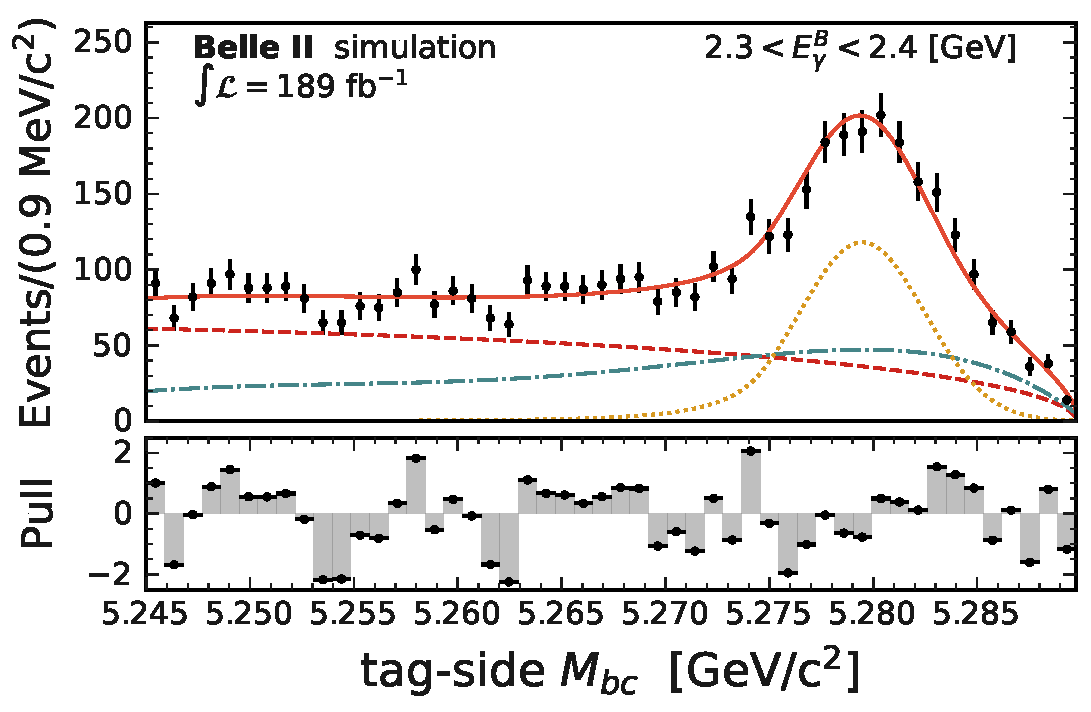
\includegraphics[width=0.3\textwidth]{figures/fitting/fits/full_MbcFit_2p3to2p4ppdf.pdf}
    }
    \subcaptionbox{\label{fig:mbc_full_2p4}}{
        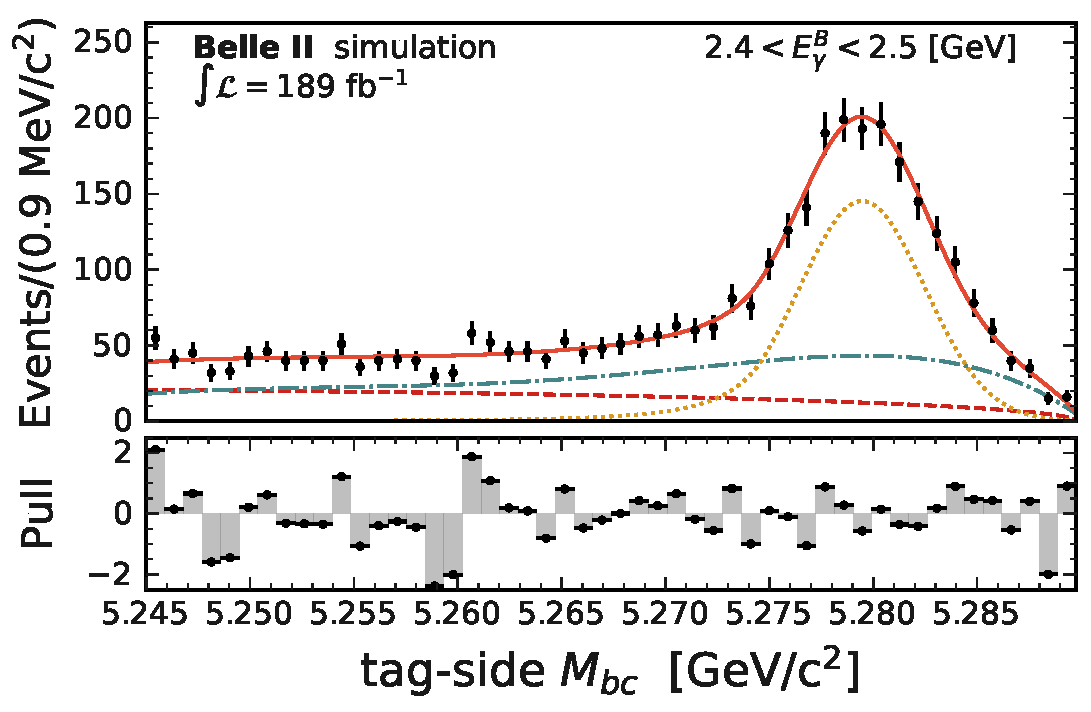
\includegraphics[width=0.3\textwidth]{figures/fitting/fits/full_MbcFit_2p4to2p5ppdf.pdf}
    }
    \subcaptionbox{\label{fig:mbc_full_2p5}}{
        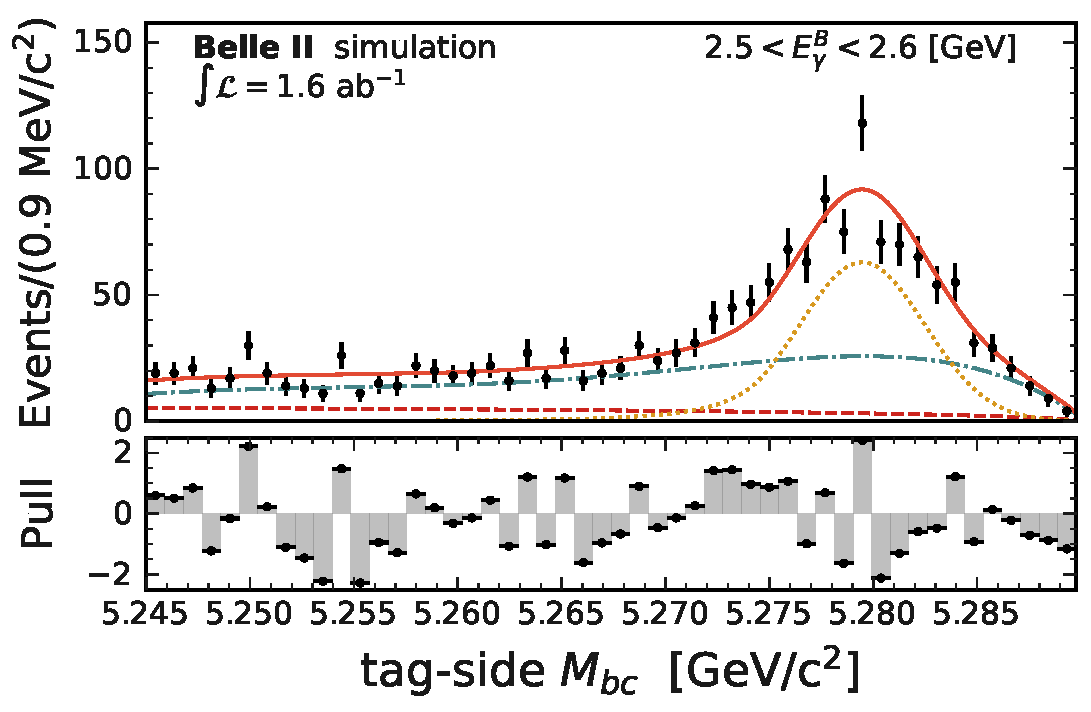
\includegraphics[width=0.3\textwidth]{figures/fitting/fits/full_MbcFit_2p5to2p6ppdf.pdf}
    }
    \subcaptionbox{\label{fig:mbc_full_2p6}}{
        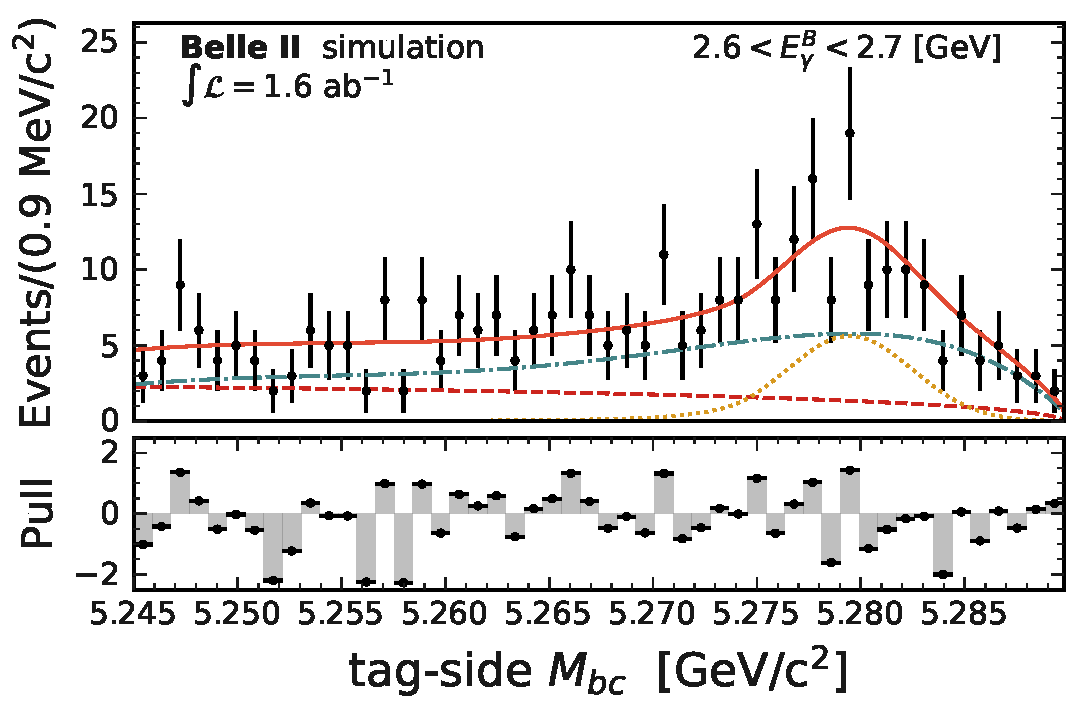
\includegraphics[width=0.3\textwidth]{figures/fitting/fits/full_MbcFit_2p6to2p7ppdf.pdf}
    }
    \subcaptionbox{\label{fig:mbc_full_2p7}}{
        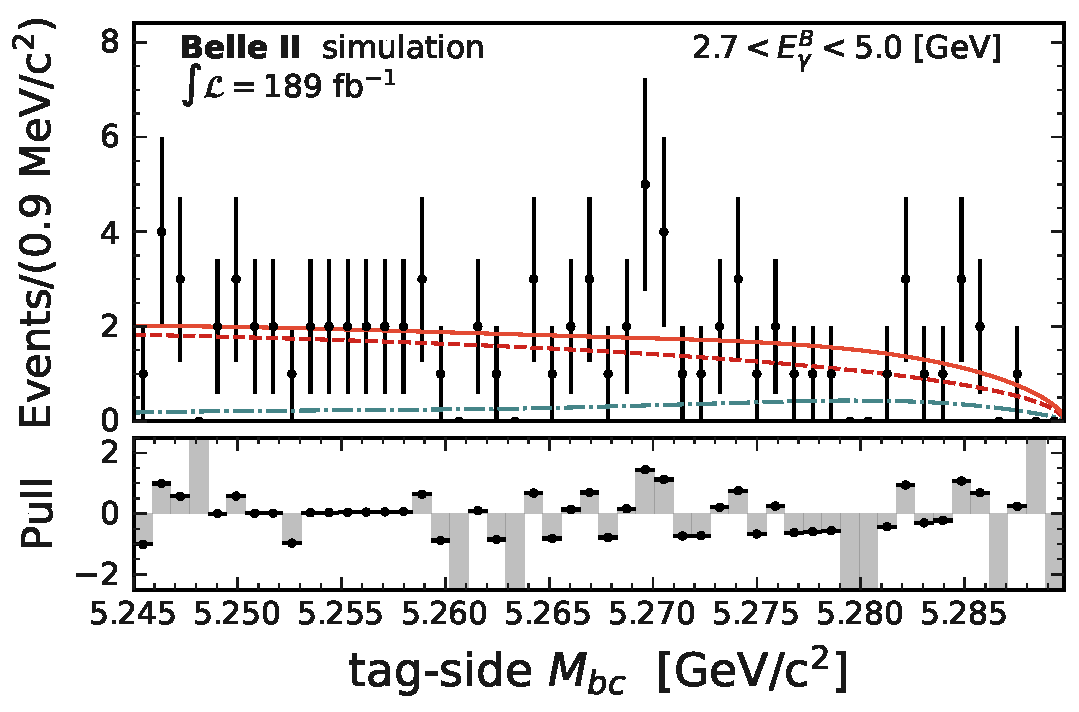
\includegraphics[width=0.3\textwidth]{figures/fitting/fits/full_MbcFit_2p7to5p0ppdf.pdf}
    }
    \caption{\label{fig:primary_full_fits}The fits on the $1.6~\invab$ dataset of generic \MC, using the fitting model from \Cref{tab:fitting_init_params}.
    Good description of the \Mbc distributions can be seen throughout the \EB bins.
    This highlights that the fit setup is able to accurately describe the simulated dataset that was used to initialise it.
    }
\end{figure}

As it was already mentioned, the main goal of the \Mbc fitter introduced in this section is to extract the good tag-\B counts in each \EB bin.
This equivalent the the normalisation parameter of the Crystal Ball \PDF -- $\mathcal{N}_{\mathrm{CB}}$.
These normalisations are shown, correspondingly to the number of good tag-\B mesons in the dataset, in \Cref{fig:generic_mc_fit_yield_comparisons}.

In the case of the rest of the other parameters -- their exact values are not needed for further analysis as long as an unbiased and accurate description of good tag-\B counts is achieved through $\mathcal{N}_{\mathrm{CB}}$.
Particularly, the main goal of including those parameters in the fitter as degrees of freedom is to ensure that the \Mbc background shape and yield estimations are sufficiently flexible to account for potential data-simulation discrepancies.
Therefore, for the rest of the thesis, other parameters will not be explicitly mentioned, unless their values become relevant for the discussion.

To ensure that the fit is receptive to changes of \BtoXsgamma signal, two simple tests are devised, where the fit is performed on generic \MC but
\begin{itemize}
    \item all \BtoXsgamma signal events are removed;
    \item \BtoXsgamma signal shape in generic \MC is reweighted using the hybrid-model weights.
\end{itemize}
The results are shown in \Cref{fig:mc_fit_yield_comparisons}.
It is clear, that if the \BtoXsgamma events are completely removed or reweighted, the \Mbc fitter presented in this Chapter responds appropriately.
This hints, but will be further explored, that although a particular simulation model was used when preparing the sample, no particular bias towards any \BtoXsgamma model is introduced.

\begin{figure}[htbp!]
    \subcaptionbox{\label{fig:generic_mc_fit_yield_comparisons}}{
        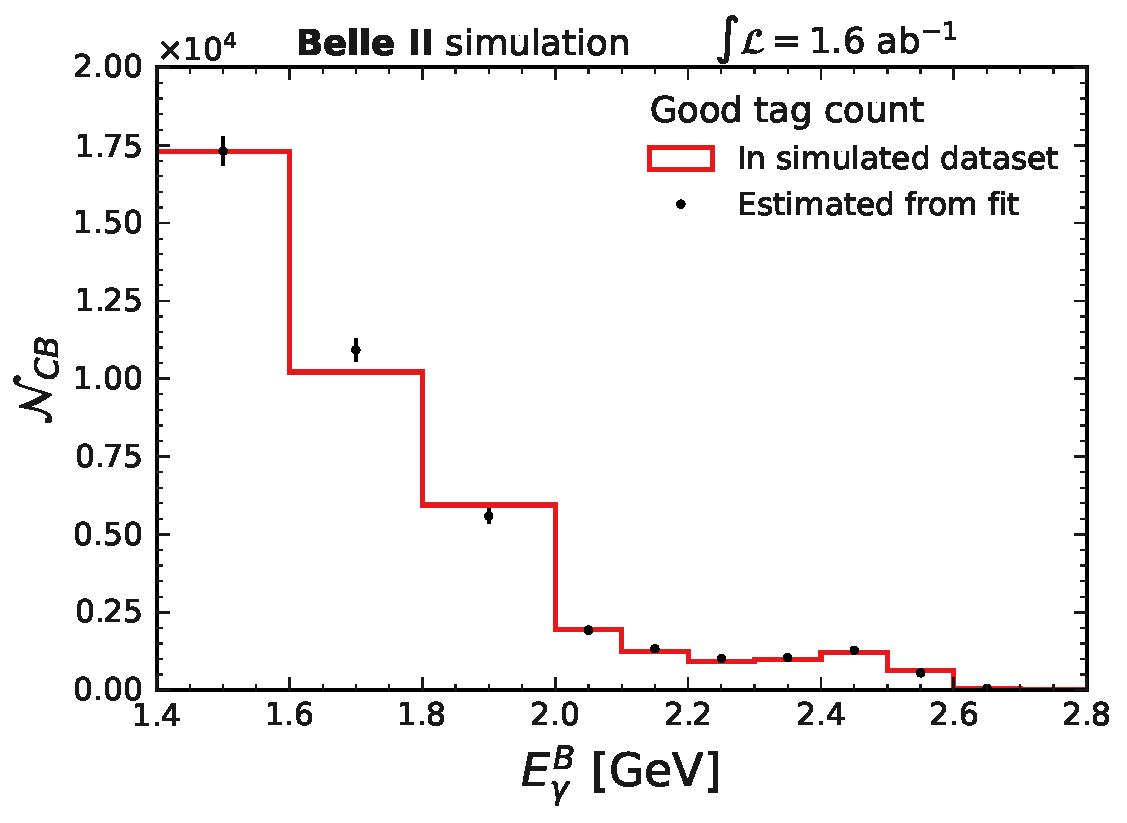
\includegraphics[width=0.3\textwidth]{figures/fitting/normal_full_fit.pdf}
    }
    \subcaptionbox{\label{fig:no_bxsgamma_mc_fit_yield_comparisons}}{
        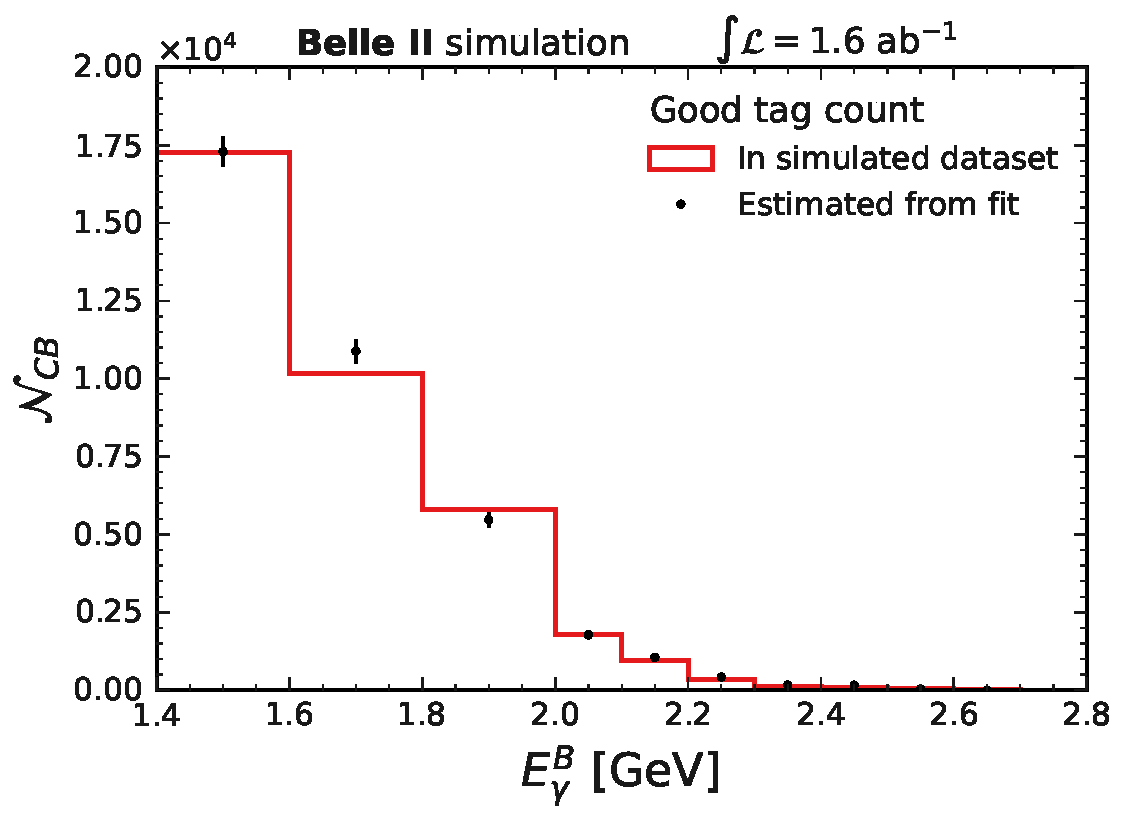
\includegraphics[width=0.3\textwidth]{figures/fitting/removed_xsgamma_full_fit.pdf}
    }
    \subcaptionbox{\label{fig:weighted_mc_fit_yield_comparisons}}{
        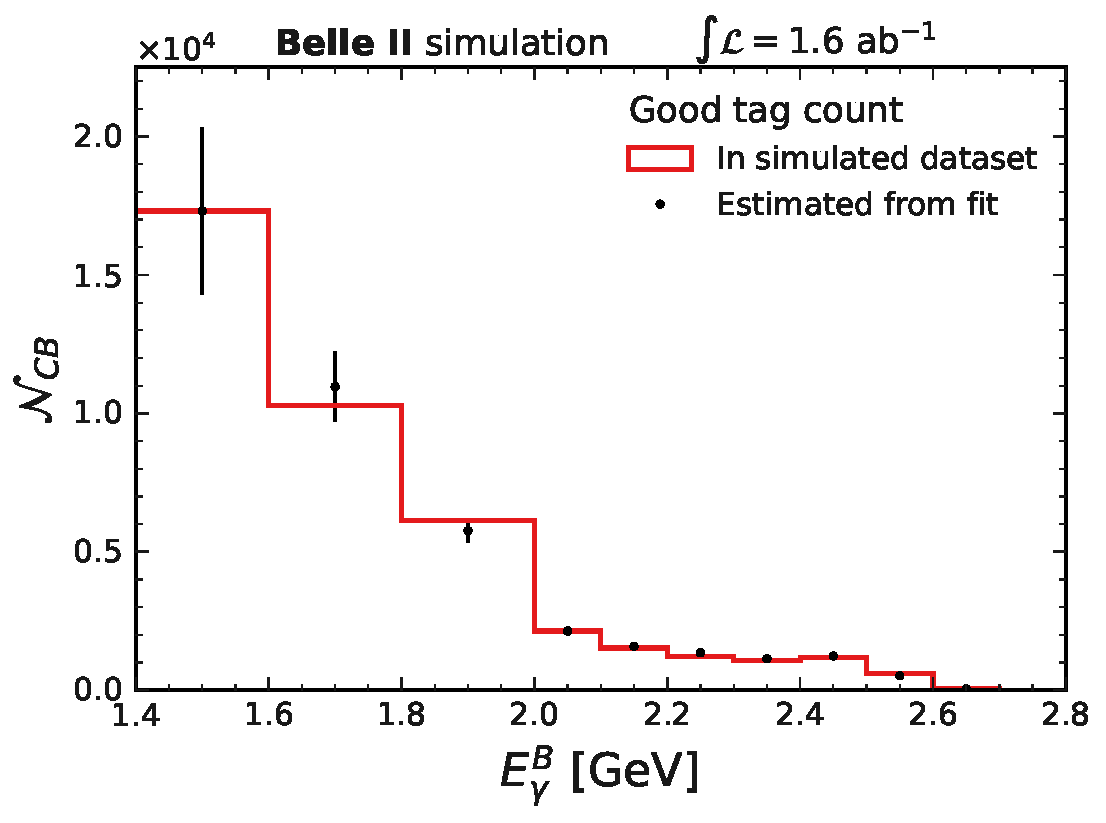
\includegraphics[width=0.3\textwidth]{figures/fitting/hybrid_weighted_full_fit.pdf}
    }
    \caption{\label{fig:mc_fit_yield_comparisons}The comparisons of estimated good tag-\B counts in each \EB bin, $\mathcal{N}_{\mathrm{CB}}$,
    for the total 1.6~\invab generic\MC dataset (\Cref{fig:generic_mc_fit_yield_comparisons}),
    for the generic \MC dataset but with all \BtoXsgamma events removed (\Cref{fig:no_bxsgamma_mc_fit_yield_comparisons}),
    and for generic \MC dataset but with hybrid-model reweighting introduced (\Cref{fig:weighted_mc_fit_yield_comparisons}).
    In each case, the uncertainties are $\texttt{HESSE}$ uncertainties estimated by the fitter.
    It can be clearly seen that the fit is receptive to the counts of the good tag-\B mesons.
    Note that the larger uncertainties in \Cref{fig:weighted_mc_fit_yield_comparisons} are due to known issues in weighted error estimation,
    and do not affect this analysis as weighted fits are not performed later.
    }
\end{figure}